
\chapter{Conceptos B\'asicos}
\noindent En  estad\'istica industrial el \'area de confiabilidad es una rama ampliamente utilizada.
Su origen se remonta a  la d\'ecada de los a\~nos 40, en aplicaciones militares durante la segunda guerra mundial. Fue empleada para estudiar el funcionamiento de equipos electr\'onicos y mec\'anicos  por periodos largos de tiempo. A partir de entonces esta rama se ha empleado dentro de empresas y negocios para la evaluaci\'on de la confiabilidad de sus componentes.\\[0.1cm]
\noindent  D\'ia con d\'ia la competencia entre productos y servicios proporcionados por empresas hacen que estas  se preocupen por la durabilidad de sus productos, pero al mismo tiempo la optimizaci\'on de sus costos. En un estudio de confiabilidad se pueden evaluar y cuantificar estos aspectos.

\noindent Desde el surgimiento de la rama de confiabilidad se han propuesto distintas definiciones, a continuaci\'on mencionaremos dos de ellas:

\begin{itemize}
\item  La confiabilidad es la probabilidad de que una unidad realice su funci\'on hasta un tiempo espec\'ifico bajo las condiciones de uso encontradas.$[{\bf \ref{me}}]$
\item La confiabilidad se refiere al funcionamiento adecuado de equipos y sistemas en el cual influye factores como software, hardware, humanos y ambientales, es decir, la probabilidad que algo funcione exitosamente bajo condiciones espec\'ificas como funci\'on del tiempo.$[{\bf \ref{law}}]$
\end{itemize} 
\noindent  Existen muchas otras expectativas de lo que deber\'ia ser  confiabilidad, pero todas ellas enfatizan, a que confiabilidad se refiere, a la calidad que tiene un sistema a trav\'es del tiempo, e involucra elementos que conllevan al mejoramiento, pron\'ostico y mantenimiento del sistema, es decir, que funcione de manera correcta durante el tiempo que sea usado y bajo las condiciones para las cuales fue creado. \\[0.2cm]


\noindent El principal an\'alisis en confiabilidad se centra en  periodos para los cuales el componente funciona, lo que com\'unmente son llamados tiempos de vida o tiempos a la falla. 

\noindent Por ejemplo, supongamos que se desea hallar la confiabilidad de  maquinas de cocer que laboran 8 horas al d\'ia. Se  observan $n$ maquinas de cocer durante un periodo de tiempo y se registran los tiempos en que fallaron o dejaron de funcionar, es decir, los tiempos de vida o 
 tiempos a la falla. Supongamos adem\'as que de las  $n$ maquinas solo $k$   maquinas fallaron y $n-k$ no fallaron, al finalizar el periodo de observaci\'on. Esta informaci\'on es proporcionada para realizar un estudio de confiabilidad. Un punto importante a recalcar es que debido a que siempre se tienen limitantes de tiempo al momento de observar el funcionamiento de componentes, es muy com\'un trabajar con datos censurados. En este contexto un dato censurado ser\'a aquella observaci\'on que nos da informaci\'on parcial de las ocurrencias de las fallas. Existen tres tipos principales de censura:
\begin{itemize}
\item Censura por la derecha: Se fija un tiempo de observaci\'on y las unidades que no fallaron son llamados censuras por la derecha.

\item Censura por la izquierda: Ocurre cuando al inspeccionar las unidades despu\'es de un periodo de tiempo se encuentra que algunas ya fallaron, pero no se sabe el momento de su ocurrencia.
\item Censura por intervalo: Cuando se inspecciona en intervalos de tiempo y se observan fallas en cierto intervalo pero no se conoce exactamente en que momento ocurrieron.
\end{itemize}



\noindent Teniendo claro que los tiempos de vida son los datos registrados del tiempo de funcionamiento de un  componente, es com\'un preguntarse la manera en que se modelan estos tiempos.  Los tiempos de vida son observaciones aleatorias que var\'ian a trav\'es del tiempo, por lo tanto son modelados por variables aleatorias. 
%Una variable aleatoria se define de la siguiente manera: 
%
%%El an\'alisis de tiempos de vida envuelve una an\'alisis de cuantiles positivos y continuos, que son los tiempos de vida para el cual el componente funciona.\\[0.2cm]
%%Los  tiempo de vida son representados por variables aleatorias:
%
%
%
%\begin{defn} 
%Sea $(\Omega, F, P)$ un espacio de probabilidad y sea $X:\Omega\rightarrow \mathbb{R}$ una funci\'on tal que $X^{-1}((-\infty,x])=\{\omega|X(\omega)\leq x\}\in F$ para todo $x$. Entonces $X$ se llama variable aleatoria.
%\end{defn}
%
%\noindent Al emplear variables aleatorias existen ciertas funciones que las caracterizan. Algunas de ellas son la funci\'on de densidad, distribuci\'on acumulada, confiabilidad y riesgo, entre otras, de las cuales podemos obtener informaci\'on valiosa acerca del fen\'omeno que se esta modelando.
%
%\begin{defn}
%Si $X$ es una variable aleatoria, la funci\'on $F:\mathbb{R}\rightarrow\mathbb{R}$ definida por $$F(x)=P(X\leq x).$$ Se llama funci\'on de distribuci\'on acumulada de $X$. Toda funci\'on de distribuci\'on satisface lo siguiente:
%\begin{enumerate}
%\item$F$ es mon\'otona y creciente.
%\item $F$ es continua por la derecha y tiene l\'imites por la izquierda.
%\end{enumerate}
%\end{defn}
%
%\noindent Existen dos tipos importantes de distribuciones: discretas y continuas.
%\noindent Para una variable aleatoria discreta $X$ definida sobre un espacio muestral $S$, la funci\'on de probabilidad satisface:
%$$P(X=x)=P(x)\geq 0,\mbox{   } x\in S,$$
%$$\sum_{x\in S} P(x)=1.$$
%
%\noindent Mientras que para una variable aleatoria continua, la funci\'on de densidad de probabilidad (fdp) esta definida como  $f:\mathbb{R}\rightarrow\mathbb{R^{+}}$ cumple:
%$$f(x)\geq 0 ,$$
%$$\int_{-\infty}^{\infty} f(x) dx=1.$$
%
%\noindent El  $p$-\'esimo cuant\'il de una variable aleatoria  $X$ es el valor $t_p$ tal que 
%$$P(X\leq t_p)=p.$$ Donde $t_p=F^{-1}(p)$. Para los tiempos de falla, $t_p$ es el tiempo al cual el 100$p\%$ de las unidades o componentes fallar\'an.[{\bf\ref{me}}]\\[0.2cm]
\noindent Dentro del an\'alisis de confiabilidad la funci\'on principal que se usa para estudiar los tiempos de vida es la funci\'on de confiabilidad.\\[0.1cm]
\noindent Si $T$ una variable aleatoria entonces la funci\'on de confiabilidad o supervivencia esta dada por:
\begin{eqnarray}\label{confiabi}
 C(t)=P(T>t)=1-F(t).
\end{eqnarray}


\noindent Donde $F$ es la funci\'on de distribuci\'on acumulada de la variable aleatoria $T$. La ecuaci\'on (\ref{confiabi})  calcula la probabilidad de que una unidad sobreviva despues de un tiempo $t$. 
\noindent La funci\'on que analiza la tasa de falla instant\'anea o la manera en la cual un componente se degrada es la funci\'on de riesgo.\\[.1cm]
Supongamos que estamos interesados en la probabilidad de que un componente que ha trabajado hasta un tiempo $t$, falle en un intervalo  $[t,t+\Delta t]$, es decir,  
\begin{eqnarray*}
P(t<T\leq t+\Delta t |T>t) =\frac{P(t<T \leq t+\Delta t )}{P(T>t)}=\frac{F(t+\Delta t )-F(t)}{C(t)}
\end{eqnarray*}


\noindent  Si deseamos conocer su tasa de falla, entonces tendremos que dividir entre la longitud del intervalo y hacerlo tender a cero, es decir,
 
\begin{eqnarray*}
h(t)&=&\lim_{\Delta t \rightarrow 0}\frac{P(t<T\leq\Delta t |T>t)}{\Delta t }\\
&=&\lim_{\Delta t \rightarrow 0}\frac{F(t+\Delta t)-F(t)}{\Delta t }\frac{1}{C(t)}\\
&=&\frac{\frac{d}{dt}F(t)}{C(t)}\\
&=&\frac{f(t)}{C(t)}
\end{eqnarray*} 
Por lo tanto la funci\'on de riesgo esta dada por:  $$h(t)=\frac{f(t)}{C(t)}.$$

\noindent Es importante ahora mencionar que dentro de la teor\'ia de confiabilidad existe una serie de distribuciones que com\'unmente se usan para modelar los tiempos de vida de los componentes. Las distribuciones m\'as comunes son la distribuci\'on Exponencial, distribuci\'on Weibull, distribuci\'on Lognormal, distrbuci\'on Log\'istica, distribuci\'on Gamma y distribuci\'on Gaussiana Inversa. La descripci\'on de ellas puede verse en {\bf [\ref{distribuciones}]}. Sin embargo en el desarrollo de esta tesina ser\'a de inter\'es considerar la distribuci\'on Weibull como veremos en cap\'itulos posteriores.
\section{Distribuci\'on Weibull}
\noindent La distribuci\'on de probabilidad Weibull fue propuesta por Waloddi Weibull  en 1951, para describir la fatiga de materiales. Hasta nuestros d\'ias es una distribuci\'on muy com\'un dentro del estudio de tiempos de vida.\\[0.1cm]
\noindent Se dice que una variable aleatoria $X$ tiene distribuci\'on Weibull, denotada como $X\sim$ Weibull$(\eta,\beta )$, si su funci\'on de densidad esta dada por:

\begin{eqnarray*}
f(t;\eta;\beta)=\frac{\beta}{\eta}\left(\frac{t}{\eta}\right)^{\beta-1}\exp\left\{-\left(\frac{t}{\eta}\right)^{\beta}\right\}
\end{eqnarray*}

\noindent donde $t>0,\beta>0$ y $\eta>0.$
\begin{figure}
\begin{center}
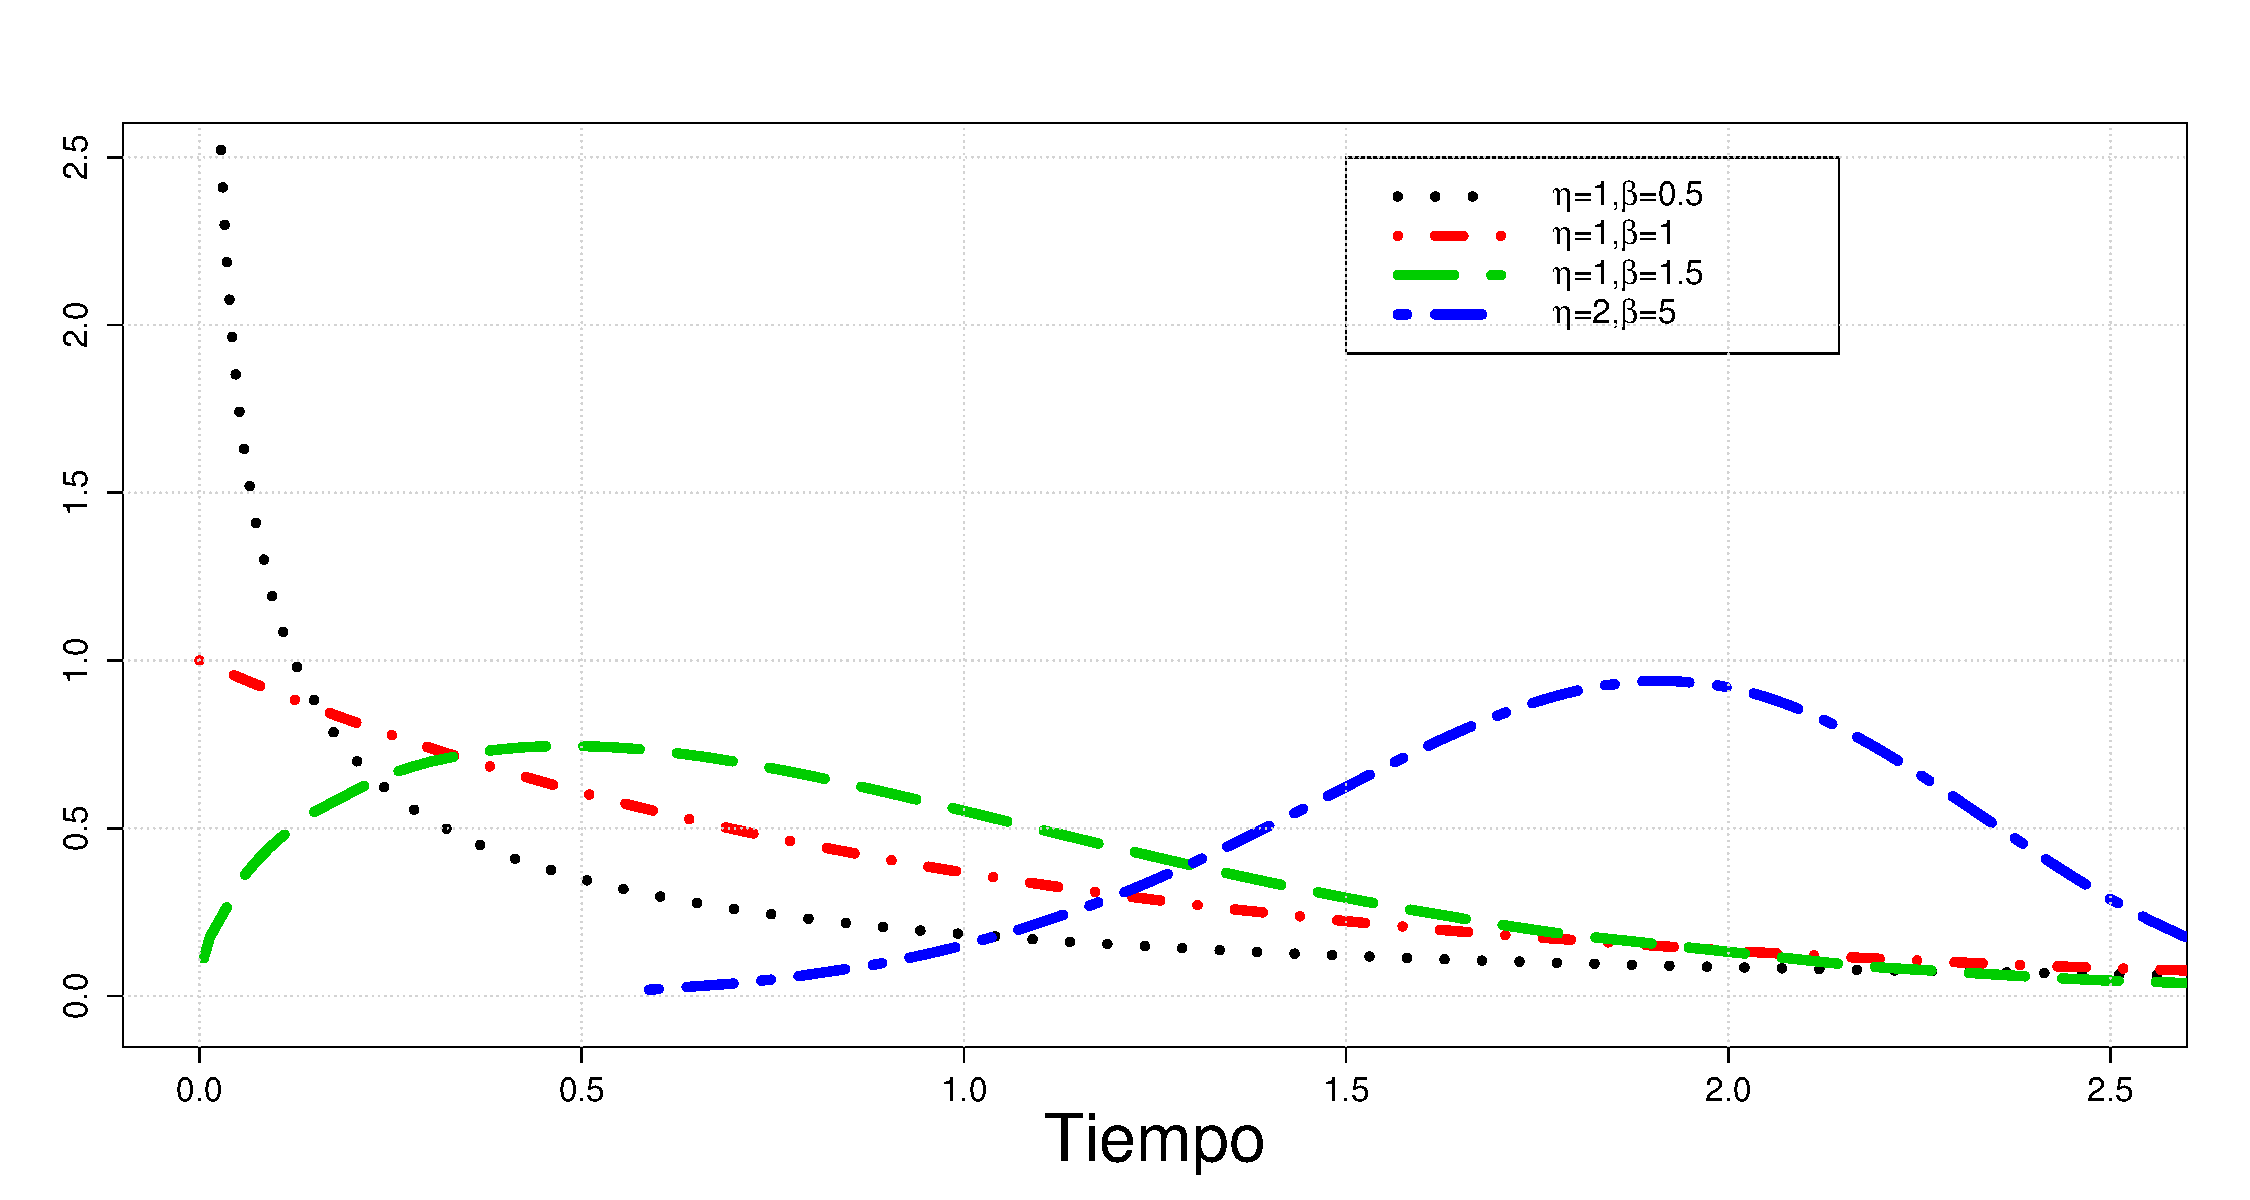
\includegraphics[scale=0.35]{weD.pdf}
\end{center}
\vspace{-1cm}\caption{\bf Comportamiento de la  densidad Weibull.}\label{wed}
\end{figure}

Entonces 

\begin{itemize}
\item Su funci\'on de distribuci\'on esta dada por:

\begin{eqnarray*}
F(t;\eta;\beta)=1-\exp\left\{-\left(\frac{t}{\eta}\right)^{\beta}\right\}
\end{eqnarray*}

\begin{figure}
\begin{center}
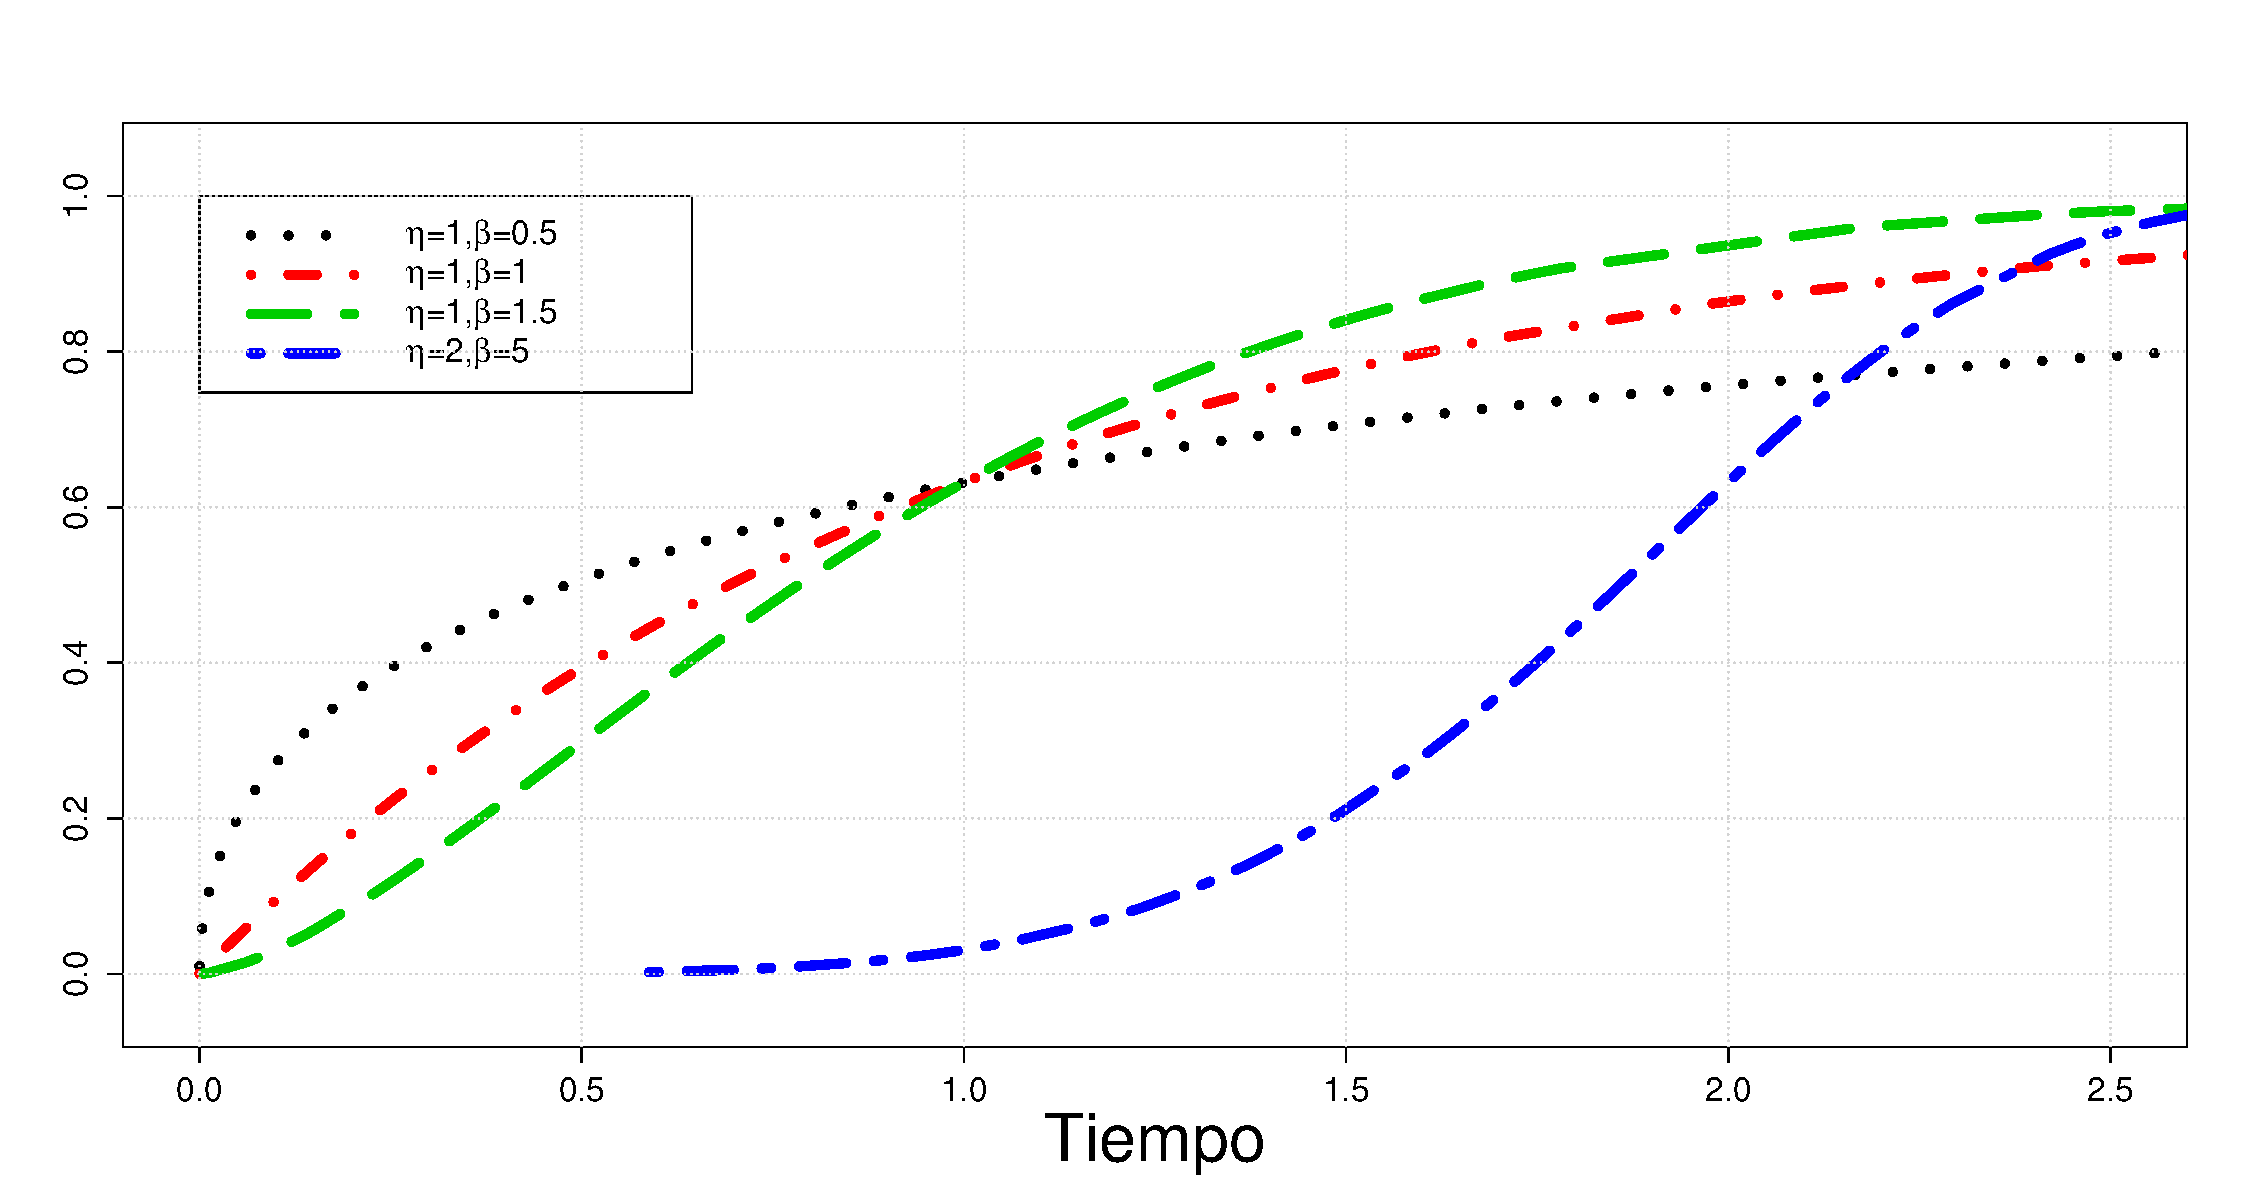
\includegraphics[scale=0.35]{weA.pdf}
\end{center}
\vspace{-1cm}\caption{\bf Comportamiento de la  funci\'on de distribuci\'on acumulada Weibull .}\label{wea}
\end{figure}


\item Su funci\'on de confiabilidad es:
\begin{eqnarray*}
C(t;\eta;\beta)=\exp\left\{-\left(\frac{t}{\eta}\right)^{\beta}\right\}
\end{eqnarray*}

\begin{figure}
\begin{center}
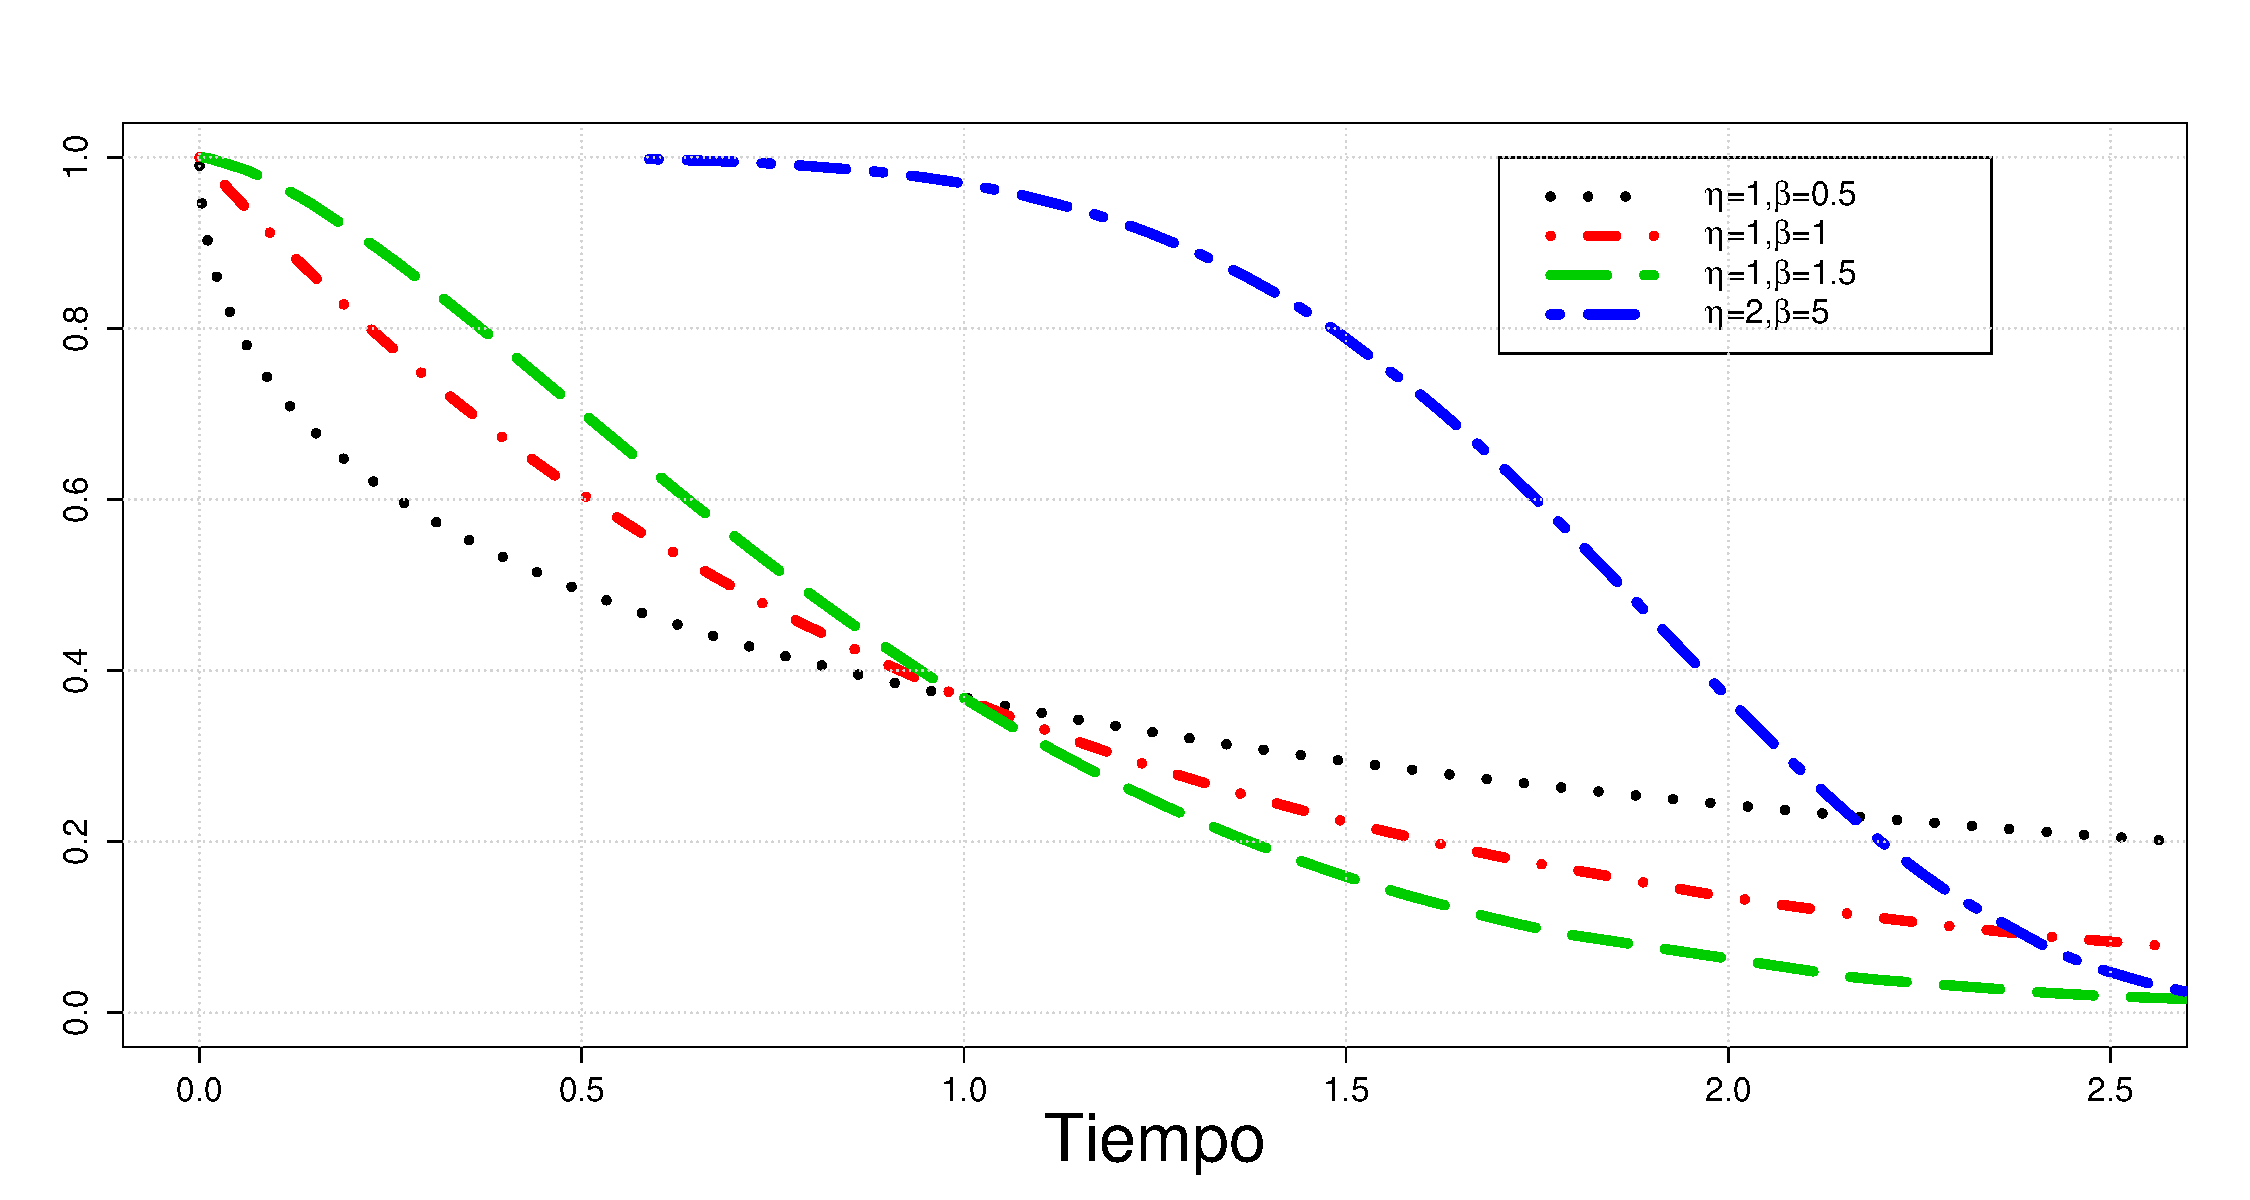
\includegraphics[scale=0.35]{weC.pdf}
\end{center}
\vspace{-1cm}\caption{\bf Comportamiento de la funci\'on de confiabilidad Weibull.}\label{wec}
\end{figure}


\item Su funci\'on de riesgo es:
\begin{eqnarray*}
h(t;\eta;\beta)=\frac{\beta}{\eta}\left(\frac{t}{\eta}\right)^{\beta-1}
\end{eqnarray*}


\begin{figure}
\begin{center}
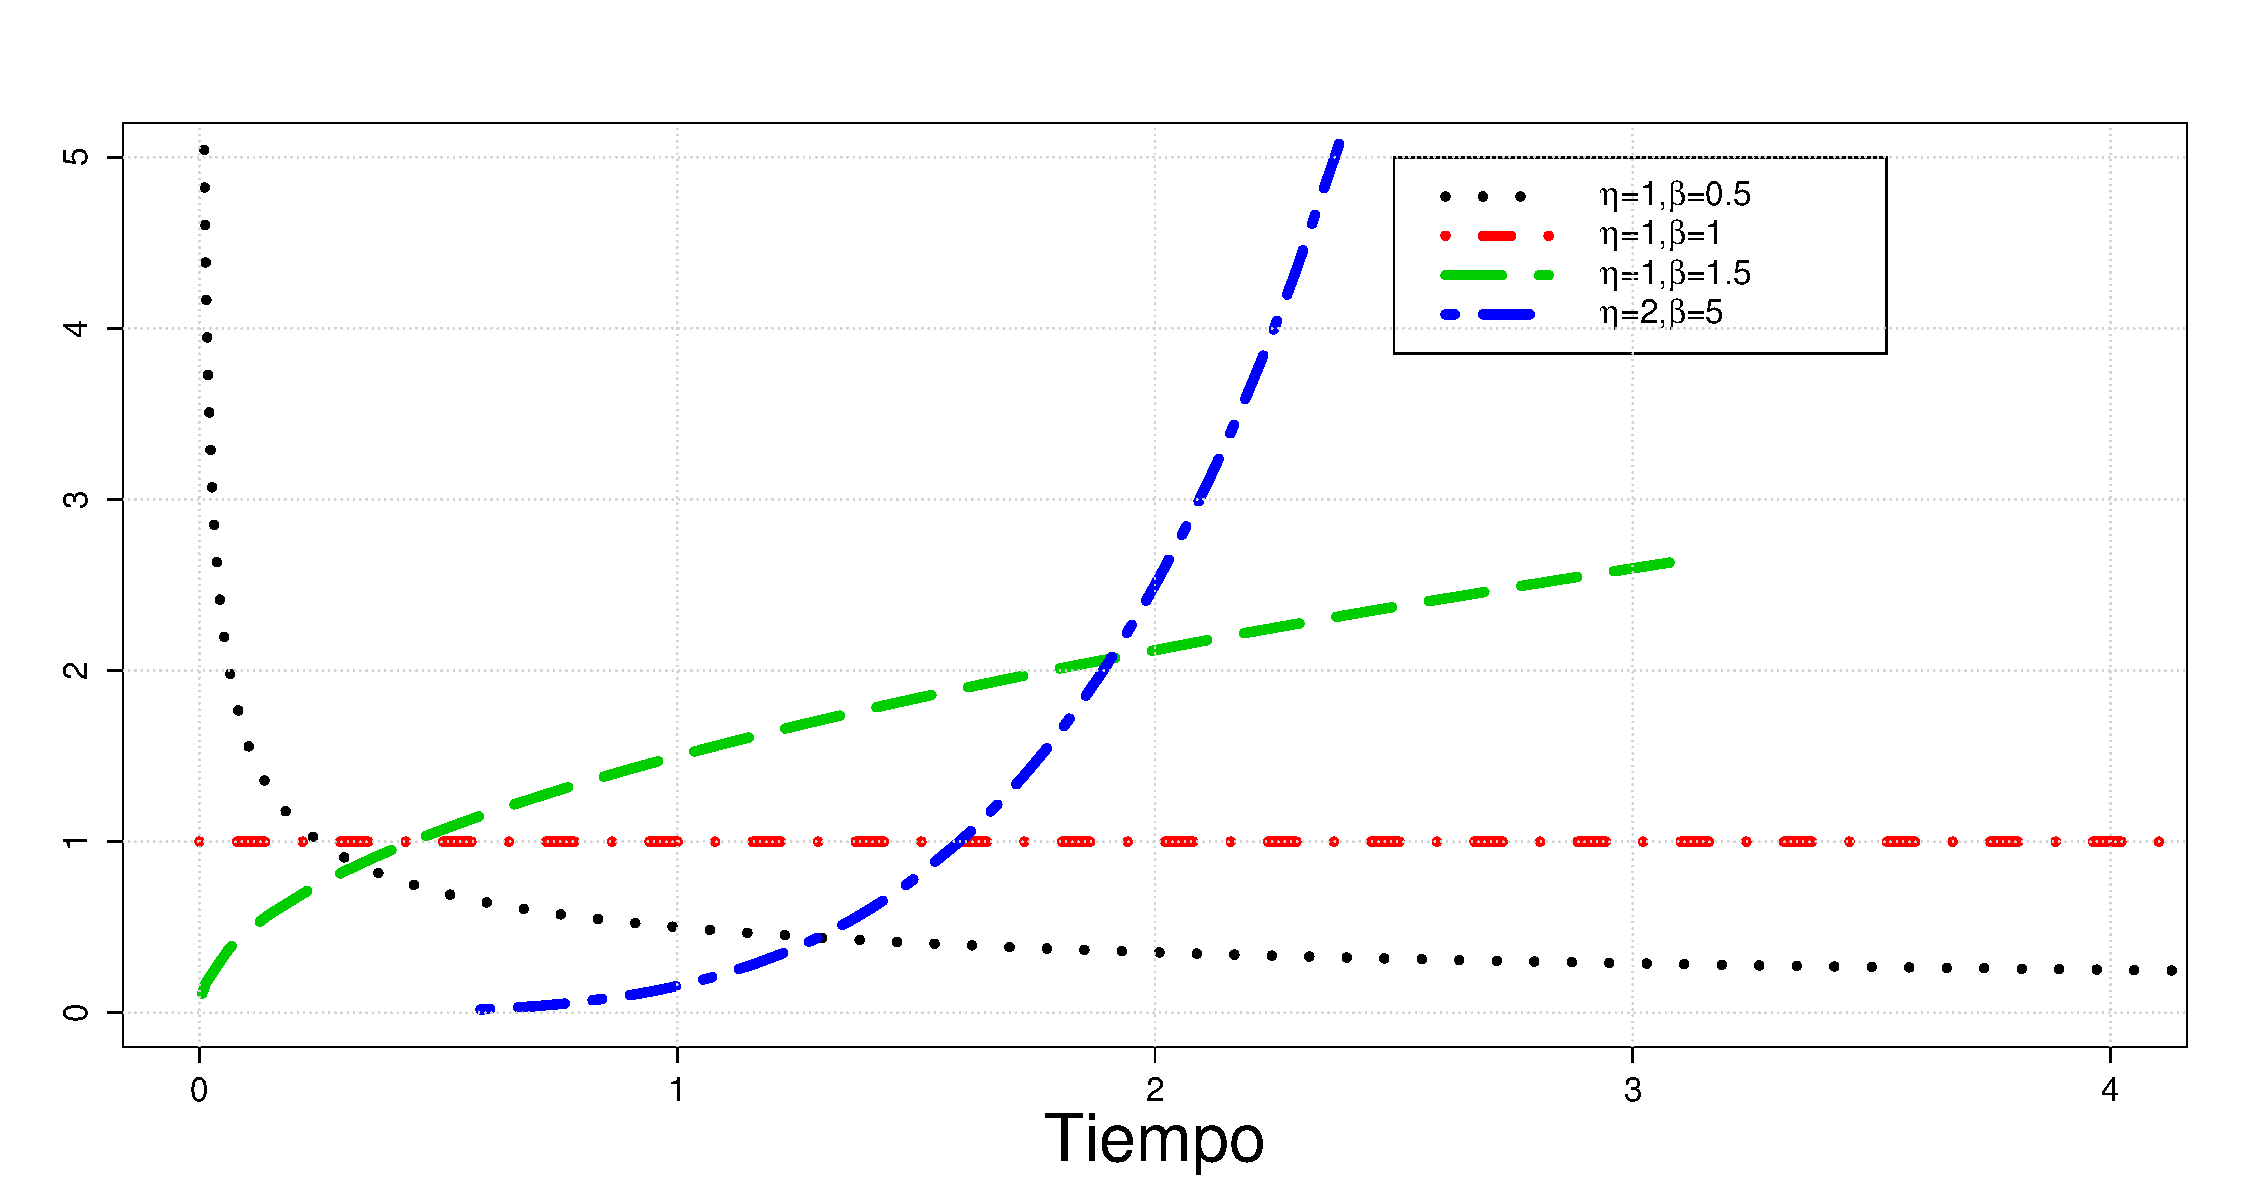
\includegraphics[scale=0.35]{weR.pdf}
\end{center}
\vspace{-1cm}\caption{\bf Comportamiendo de la funci\'on de riesgo Weibull.}\label{wer}
\end{figure}
\end{itemize}

\noindent En las Figuras \ref{wed},  \ref{wea},  \ref{wec} y  \ref{wer} podemos ver distintas formas de la distribuci\'on Weibull en cuanto a su densidad, distribuci\'on acumulada, confiabilidad y funci\'on de riesgo.
Donde $\eta$  representa el par\'ametro de escala y $\beta$ el de forma. A $\eta$ tambi\'en se le llama vida caracter\'istica, ya que coincide con el cuantil $t_{.63}$, el cual se encuentra despu\'es de la mediana y  describe la mayor parte de la vida de componente. Esta distribuci\'on es ampliamente usada dada la flexibilidad que tiene su funci\'on de riesgo, puesto que para valores de $\beta<1$ se tiene una funci\'on de riesgo decreciente, para $\beta=1$ es constante y para $\beta>1$ es creciente como se aprecia en la  Figura \ref{wer}. 


\section{Introducci\'on al uso de M\'etodos Bayesianos}

\noindent La estad\'istica Bayesiana  combina los datos del experimento a analizar con informaci\'on previa, que se conoce o se ha observado previamente de dicho experimento llamada distribuci\'on a priori, para producir una distribuci\'on posterior de los par\'ametros. \\[0.1cm]
%esq44.pdf
\begin{figure}
\begin{center}
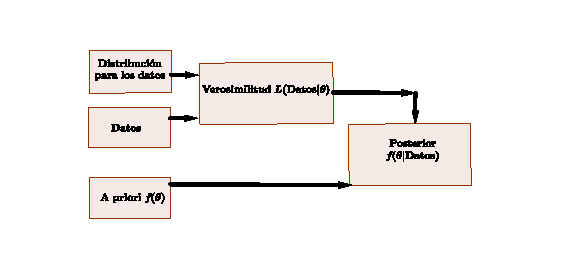
\includegraphics[scale=1.8]{bayes1.pdf}
\end{center}
\vspace{-2cm}\caption{\bf M\'etodo Bayesiano para realizar inferencia.}\label{eb}
\end{figure}
\noindent Las combinaciones de experiencias pasadas dan la informaci\'on a priori para formar un marco de referencia y tomar una decisi\'on que conlleve al mejoramiento de alg\'un proceso. En la mayor\'ia de las aplicaciones es necesario y \'util combinar informaci\'on a priori con datos experimentales. Por ejemplo,  supongamos que al realizar un estudio de confiabilidad los ingenieros expertos saben con cierta certeza, el tiempo promedio que tarda en fallar un componente.  
Adem\'as de  estudios anteriores, su tiempo de falla es Weibull con ciertos par\'ametros que se encuentra dentro de un rango espec\'ifico. Para estimar la distribuci\'on del ciclo de vida de un componente similar, este conocimiento previo puede ayudar a optimizar el  tama\~no de la muestra y a disminuir la incertidumbre  en la inferencia.


\noindent  A grandes rasgos el procedimiento para hacer inferencia Bayesiana sobre un vector de par\'ametros $\theta$, es el siguiente (Figura \ref{eb}):

\begin{itemize}
\item Conocimiento apriori acerca de $\theta$ expresado en t\'erminos de una funci\'on de densidad de probabilidad, denotada por $f(\theta)$.
\item La verosimilitud para los datos disponibles y un modelo especificado dado por $L(Datos|\theta)$.
\item Utilizar la regla de Bayes, para obtener una distribuci\'on posterior, que resulte de la combinaci\'on de la verosimilitud y el conocimiento de la distribuci\'on a priori de $\theta$. La distribuci\'on posterior es usada para cuantificar la incertidumbre de las cantidades de inter\'es.  
\end{itemize}
 

\noindent Uno de los primeros pasos para hacer estad\'istica Bayesiana consiste en obtener informaci\'on modelable en t\'erminos de una funci\'on de densidad.
La obtenci\'on de la distribuci\'on a priori para un solo par\'ametro puede ser sencilla, si se ha considerado la experiencia en situaciones similares. Para un vector de par\'ametros, establecer la distribuci\'on a priori conjunta puede ser mucho m\'as complicado. Tambi\'en es dif\'icil obtener informaci\'on sobre la dependencia de los par\'ametros y expresarlo en t\'erminos de una distribuci\'on conjunta. Por ejemplo, si la experiencia previa  de estimaciones pasadas para los par\'ametros de la distribuci\'on  lognormal $\mu$ y $\sigma$ indican que est\'an altamente correlacionados, significa que la distribuci\'on a priori para estos par\'ametros deber\'ia reflejar esta dependencia


\noindent Un enfoque adecuado para construir la distribuci\'on a priori, consiste en formular informaci\'on acerca de un cuantil en especial (o par\'ametros), de acuerdo a experiencia previa.\\[0.2cm]

\noindent  Al momento de elegir una distribuci\'on a priori, existen 3 tipos diferentes:
 \begin{itemize}
 \item Cuando se tiene la informaci\'on suficiente tales que los par\'ametros son conocidos, y conducen a una distribuci\'on degenerada\footnote{Una variable aleatoria $X$ es degenerada en un punto o conjunto $c\in \mathbb{R}$, si $P(X=x)=1$ si $x\in c$ y $P(X=x)=0$ si  $x\notin c.$}. 
 \item Informaci\'on difusa de los par\'ametros, que conduzcan una distribuc\'ion a priori no informativa.
 \item Una distribuci\'on a priori informativa no degenerada.
 \end{itemize}
 
 
\noindent Comunmente, las principales fuentes de informaci\'on para una distribuci\'on a priori son:
 
 \begin{enumerate}
 \item Opini\'on de expertos u otros.
 \item Informaci\'on de datos pasados.
 \end{enumerate}
 
\noindent  Finalmente podemos mencionar que el uso de una distribuci\'on a priori es un instrumento de modelaci\'on que permite descartar entornos o escenarios improbables. Este  instrumento de modelaci\'on  permite tomar una decisi\'on acerca de la forma que debe tener la funci\'on de distribuci\'on a priori.

\section{Inferencia Bayesiana}

\noindent Se puede observar que dadas dos variables aleatorias $X$, $Y$, la funci\'on de densidad $f(Y|X)$ es proporcional a $f(X,Y)$, en el siguiente sentido. Sabemos que
 $$f(y)=\int f(x,y)\,dx=\int f(x)f(y|x)\,dx,$$
 es claro que 
\begin{eqnarray}
f(y|x)=\frac{f(x,y)}{f(x)}=\frac{f(y)f(x|y)}{f(x)}.\label{pro}
\end{eqnarray}
Entonces $$f(Y|X)\propto f(Y)f(X|Y),$$
esta es una de las formas del teorema de Bayes y es la utilizada dentro de la estad\'istica Bayesiana. La igualdad esta bien definida para variables discretas y continuas  {\bf  [\ref{PL}]}. La constante
 de proporcionalidad, es el denominador de la expresi\'on (\ref{pro}), y es necesaria para que $f(Y|X)$ sea una distribuci\'on de probabilidad. En el caso continuo se determina por

$$\frac{1}{f(x)}=\frac{1}{\int f(x,y)\,dy},$$y en el caso discreto es 
$$\frac{1}{f(x)}=\frac{1}{\sum_{y} f(x,y)}.$$



\noindent Veamos un ejemplo artificial de la manera en la cu\'al se aplica el teorema de Bayes.

\subsubsection{Ejemplo}
\noindent Supongamos que $Y$ es la variable aleatoria que describe el tiempo en que falla por primera vez cierto objeto {\bf  [\ref{PL}]}, el cual es medido por un instrumento que tiene un peque\~no retraso en  la medici\'on. Sea $X$ el tiempo de registro del instrumento, es decir, X es mayor que Y, pero solo es posible observar $X$ y necesitamos concluir algo acerca de $Y$. Supongamos adem\'as que se sabe que
\begin{eqnarray*}
f(y)&=&\exp\{-y\} \mbox{  } (0<y<\infty)\\
f(x|y)&=&k\exp\{-k(x-y)\}  \mbox{  } (y<x<\infty)
\end{eqnarray*}

\noindent Entonces para hacer conclusiones del comportamiento de $Y$ dado $X$, necesitamos a  $f(Y|X)$. Aplicando el teorema de Bayes citado anteriormente se tiene que
\begin{eqnarray*}
f(y|x) &\propto& f(y)f(x|y)\\
&\propto& k\exp\{-y\}\exp\{-k(x-y)\} \\
&\propto& \exp\{(k-1)y\}  \mbox{  } (0<y<x).
\end{eqnarray*}

\noindent Con frecuencia es suficiente con obtener este resultado, pero la constante de proporcionalidad es necesaria para que lo que se esta obteniendo sea un distribuci\'on de probabilidad, en este caso la constante de proporcionalidad es:

\begin{eqnarray*}
\int_{0}^{x}  \exp\{(k-1)y\}dy &=& \frac{1}{k-1}\left[\exp\{(k-1)x\}-1\right].
\end{eqnarray*}
\newpage

\noindent Si estamos interesados en $k$ par\'ametros desconocidos $$\theta=(\theta_1,\theta_2,\cdots,\theta_k)$$ y tenemos la creencia de alguna distribuci\'on a priori para estos valores expresada en t\'erminos de la distribuci\'on de probabilidad $f(\theta)$, contamos con $n$ observaciones de una muestra del experimento a observar $$X=(x_1,x_2,\cdots,x_n)$$
con una distribuci\'on de probabilidad que depende de estos $k$ par\'ametros desconocidos. Entonces los componentes de $X$ son variables aleatorias y la dependencia de $X$ sobre $\theta$,  puede ser expresada en t\'erminos de una funci\'on de densidad de probabilidad (fdp) $$f(X|\theta).$$

\noindent Es posible encontrar una manera de expresar la distribuci\'on de inter\'es considerando la distribuci\'on a priori y los datos. La herramienta b\'asica es el teorema de Bayes para variables aleatorias, este afirma que

$$f(\theta|X)\propto f(\theta)f(X|\theta),$$
la funci\'on $f(X|\theta)$, como funci\'on de $X$ y fijando $\theta$ es una densidad, sin embargo $f(X|\theta)$ como funci\'on de $\theta$ la llamamos funci\'on de verosimilitud y con frecuencia la escribimos como $$L(\theta|X)=f(X|\theta).$$

\noindent Con $f(\theta)$ como la distribuci\'on a priori para $\theta$ y $f(\theta|X)$ como la distribuci\'on posterior para $\theta$ dado $X$, el teorema de Bayes se transforma en su forma m\'as memorable:
 
\begin{center}
\begin{tabular}{|c|}
\hline
Posterior $\propto$ A priori $\times$ Verosimilitud.\\
\hline
\end{tabular}
\end{center}


\noindent La relaci\'on anterior resume, el camino en el cual deber\'iamos modificar nuestra creencia considerando los datos disponibles. Para una muestra inicial de $X$ observaciones 
\begin{eqnarray}
f(\theta|X)\propto f(\theta)L(\theta|X).\label{poscita}
\end{eqnarray}
\noindent Los c\'alculos y conclusiones anteriores se sintetizan en el siguiente teorema.
\begin{thm}
La distribuci\'on posterior $f(\theta|X)$ es la distribuci\'on condicional de $\theta$ dado los datos, expresada por:

\begin{eqnarray*}
f(\theta|X)&=&\frac{L(X|\theta)f(\theta)}{\int_{\Omega} L(X|\theta)f(\theta)\,d\theta},
\end{eqnarray*}
donde $\Omega$ es el espacio param\'etrico de $\theta$ y $f(\theta)$ es la distribuci\'on a priori para  $\theta$.\\[0.2cm]
De aqu\'i:
$$f(\theta|X)\propto L(X|\theta)f(\theta)$$
y
$$f(X)=\int L(X|\theta)f(\theta)\,d\theta,$$
a esta \'ultima expresi\'on se le suele llamar verosimilitud integrada. Es en realidad la distribuci\'on marginal de los datos, vista como funci\'on de $X$.
\end{thm}

\noindent La distribuci\'on posterior es  una distribuci\'on para los par\'ametros de la distribuci\'on y en la mayor\'ia de las veces es de inter\'es hacer inferencia sobre alguna observaci\'on $X$, y no sobre los par\'ametros. Para realizar esta inferencia se emplea la distribuci\'on predictiva.

 \begin{thm}
 Bajo el supuesto de que existe independencia entre los datos $X$, dados los par\'ametros $\theta$, para la observaci\'on futura $y$, la distribuci\'on predictiva posterior es:
 $$f(y|X)=\int_{\theta} f(y|\theta)f(\theta|X) d\theta=E_{(\theta|X)}[f(y|\theta)],$$
 \end{thm}

\noindent La demostraci\'on del teorema anterior se puede ver en Bernando y Smith(1994). [{\bf \ref{BT}}]\\[0.1cm]
\noindent El ejemplo siguiente ilustra la forma de realizar inferencia sobre los par\'ametros de una distribuci\'on.

\subsubsection{Ejemplo}
\noindent Supongamos que lanzamos de una moneda  no justa y observamos el resultado. Modelamos el experimento con variables aleatorias Bernoulli de par\'ametro $p$, $x_i\sim$Ber ($p$). Dado que es una moneda no justa, tenemos conocimiento a priori de $p$, modelada como una variable aleatoria Beta, $p\sim$Beta$(\alpha, \beta)$. Para deducir conclusiones acerca de este experimento necesitamos hallar la distribuci\'on posterior de $p$ dado los datos, utilizando la expresi\'on (\ref{poscita}).\\


\noindent La verosimilitud esta dada por
\begin{eqnarray} \label{vee}
f(X|p)= p^{\sum x_i}(1-p)^{n-\sum x_i}.
\end{eqnarray}
La distribuci\'on a priori de $p$ es: 
\begin{eqnarray} \label{ap}
f(p)=\frac{\Gamma(\alpha)\Gamma(\beta)}{\Gamma(\alpha + \beta)} p^{\alpha-1}(1-p)^{\beta-1}\mbox{I}_{[0,1]}(p)
\end{eqnarray}

La distribuci\'on posterior usando (\ref{vee}),  (\ref{ap}) y sustituyendolas en (\ref{poscita}) es
\begin{eqnarray*} 
f(p|X)&\propto& f(X|p)f(p)\\
&\propto& p^{\sum x_i +\alpha-1}(1-p) \mbox{I}_{[0,1]}(p),
\end{eqnarray*}
esta \'ultima expresi\'on puede ser completada para que sea una distribuci\'on Beta, por lo tanto 

$$p|X\sim \mbox{Beta} (\alpha + \sum x_i, \beta+n-\sum x_i).$$

\noindent La distribuci\'on posterior encontrada pertenece a la misma familia que la distribuci\'on a priori. Cuando se tienen casos como los anteriores en donde la distribuci\'on a priori y la posterior se distribuyen de la misma manera pero con diferentes par\'ametros son llamadas distribuciones conjugadas.


%
%\subsection{Distribuci\'on predictiva}
%
%En muchas de las aplicaciones necesitamos calcular  la distribuci\'on marginal 
%$$p(X)=\int p(X|\theta)p(\theta)\,d\theta$$
%la cual es llamada distribuci\'on predictiva de $X$.

%Cualquier informaci\'on emp\'irica, combinada con el conocimiento que ya se tenga del problema que se estudia y actualiza dicho conocimiento.

%
%\subsection{Familias conjugadas}
%
%Tanto $p(\theta)$ como $p(\theta|x)$ son distribuciones de probabilidad sobre $\theta$: como sabemos la primera incorpora informaci\'on a priori y la segunda actualiza dicha informaci\'on muestral que se puede obtener. Si bien dijimos que la elecci\'on de una u otra distribuci\'on de probabilidad  para modelar nuestra incertidumbre sobre $\theta$ no resulta crucial en tanto sea factible e licitar con cualquiera de ellas una distribuci\'on a priori, resulta conveniente que $p(\theta)$ y $p(\theta|x)$ pertenezcan a la misma familia.
%\\[0.3cm]
%
%Definici\'on: Sea $P:=\{p(x|\theta): \theta \in \Omega\}$ una familia param\'etrica. Una clase (o colecci\'on) de distribuciones de probabilidad $F$ es una familia conjugada para $P$ si para todo $p(x|\theta)\in P$ y $p(\theta)\in F$ se cumple que $p(\theta|x)\in F$.\\[0.2cm]
%
%Uno de los principales objetivos de la teor\'ia de decisi\'on en el desarrollo de procesos l\'ogicos para la toma de decisiones bajo condiciones de incertidumbre. La idea es plantear los problemas  de inferencia estad\'istica como problemas de decisi\'on y aprovechar por tanto los resultados que ya se tienes respecto a esto ultimo.
%\\[0.2cm]
%Al momento de resolver un problema de decisi\'on existen diversas formar que nos interesa para hacer inferencia desde el enfoque bayesiano y para ello requerimos tener identificado lo siguiente:
%
%\begin{itemize}
%\item El espacio de estados $\Omega$.
%\item Una funci\'on de probabilidad $P$ sobre los elementos de $\Omega$,
%\item Una funci\'on de utilidad $u$ sobre $C$.
%\end{itemize}
%
%


\subsection{M\'etodo de Simulaci\'on}
\noindent Antes de la aparici\'on de m\'etodos computacionales las distribuciones conjugadas eran las empleadas en estad\'istica Bayesiana, por la facilidad de los c\'alculos. Sin embargo limitaba en gran medida el manejo de las distribuciones a priori y de los posibles modelos. Actualmente los procedimientos computacionales han realzado el empleo de este enfoque estad\'istico, puesto que se puede proponer la distribuci\'on a priori adecuada, sin forzarla a que sea necesariamente conjugada, permitiendo que al momento de obtener la distribuci\'on posterior, aunque se tenga una expresi\'on bastante compleja,  puedan obtenerse  aproximaciones de esta distribuci\'on. Estas aproximaciones se ven reflejadas en la simulaci\'on de datos de la distribuci\'on posterior. A finales de los a\~nos 80's surgieron m\'etodos de simulaci\'on para realizar c\'alculos de este tipo, uno de los m\'as utilizados son los algoritmos Markov Chains Monte Carlo (MCMC).\\[0.1cm]
\noindent El algoritmo MCMC (Markov Chain Monte Carlo) es una clase general de algoritmos usados para producir muestras de la distribuci\'on posterior, en altas dimensiones. El objetivo b\'asico de un algoritmo MCMC es simular valores o muestras de una distribuci\'on posterior  de un vector de par\'ametros. Tiene la propiedad de que la distribuci\'on de la $j$-\'esima iteraci\'on en la secuencia de valores muestrales, convergen a una muestra aleatoria de la distribuci\'on posterior para $j$ grande. En general muestras sucesivas de la distribuci\'on posterior est\'an correlacionadas, pero esta correlaci\'on tiende a perderse conforme el tama\~no de la muestra crece. As\'i para valores grandes de la muestra se actualizan los \'ultimos grupos dentro de una secuencia, digamos $\theta^{(m)}$, $\theta^{(m+1)} \cdots \theta^{(m+k)}$ y estos representan la muestra de la distribuci\'on posterior de inter\'es.\\[0.1cm]
\noindent Consideremos dos tipos de algoritmos MCMC: Metropolis- Hasting y Gibbs samplers. A continuaci\'on mencionaremos las ideas b\'asicas de estos algoritmos.

\subsubsection{ Muestreo Gibbs.}
\noindent El muestreo Gibbs  es probablemente uno de los algoritmos MCMC m\'as usados dentro de la estad\'istica Bayesiana [{\bf \ref{mi}}]. El t\'ermino formal fue establecido por  Geman y Geman[{\bf \ref{geman}}], cuando estudiaban modelos de procesamiento de im\'agenes. El muestreo Gibbs es un m\'etodo para generar datos de variables aleatorias sin tener que realizar expl\'icitamente los c\'alculos que se  involucran para obtener la densidad, se basa en propiedades de las cadenas de Markov.
Cassella y George(1992) dan una tutorial acerca de este m\'etodo [{\bf \ref{gibbs}}].\\[0.12cm]
\noindent  A grandes rasgos un Muestreo Gibbs se construye de la siguiente manera.\\[0.1cm]
\noindent Supongamos que tenemos un vector de par\'ametros 
$\theta=(\theta_1,\cdots,\theta_q)$ y denotamos las distribuciones posteriores condicionales totales (full conditionals) por :\\
$f_1(\theta_1|\theta_2,\cdots,\theta_q,datos)$, 
$f_2(\theta_2|\theta_1,\theta_3\cdots,\theta_q,datos)$, 
$\cdots $, $f_q(\theta_q|\theta_1,\cdots,\theta_{q-1},datos)$.


\begin{description}
\item[PASO I:] Generar un valor inicial $\theta^{0}=(\theta_1^{0},\cdots,\theta_p^{0})$ y considerar j=0.

\item[PASO II:]
Construir $\theta^{j+1}=(\theta_1^{j+1},\cdots,\theta_p^{j+1})$ de la siguiente manera:
\begin{itemize}
 \item Generar $\theta_1^{j+1} \sim f_1(\theta_1|\theta_2,\cdots,\theta_q,datos)$;
 \item Generar $\theta_2^{j+1}\sim f_2(\theta_2|\theta_1,\cdots,\theta_q,datos)$ $\cdots$
 \item Generar $\theta_{q}^{(j+1)}\sim f_q(\theta_q|\theta_1,\cdots,\theta_{q-1},datos).$ 
\end{itemize}
\item[PASO III:] incrementar $j$ y regresar al paso II.
\item[PASO IV:] Regresar $\{\theta^{(1)},\theta^{(2)}\cdots \theta^{(M)}\}$
\end{description}

\noindent Gelfand y Smith (1992) mostraron que bajo ciertas condiciones de regularidad, el vector generado  tiene distribuci\'on estacionaria $f(\theta|Datos)$ utilizando ciertas propiedades de cadenas de Markov.

\subsubsection{Metropolis Hastings}
\noindent Las primeras ideas del algoritmo Metropolis-Hastigs fueron introducidas en el art\'iculo
``The Monte Carlo Method'' por Metropolis and Ulam(1949), mostrando un ejemplo de estimaci\'on de probabilidades de \'exito para una estrategia del solitario, realizando muchos intentos y   calculando la proporci\'on de \'exito. El m\'etodo fue generalizado y probado m\'as tarde por el profesor de la universidad de Toronto  llamado W. Keith Hasting(1970). David B. Hitchcock(2003) proporciona una historia detallada sobre el nacimiento de este m\'etodo. {\bf [\ref{MH}}]

\noindent Metropolis Hasting es un algoritmo de simulaci\'on al igual que Muestro Gibbs, solo que un poco m\'as general. Su mayor peso recae en la selecci\'on de una distribuci\'on propuesta.
\noindent Supongamos que $\pi(x)$ es la distribuci\'on objetivo, por ejemplo, es la distribuci\'on posterior, de la que se desea simular. La distribuci\'on ``propuesta'' es una distribuci\'on condicional $q(y|x)$ y constituye ``una sugerencia'' de pasar de un estado $x$ a  un punto $y$. [{\bf \ref{UMH}}]\\
\noindent De manera general el algoritmo es el siguiente [{\bf \ref{mi}}]: 

\begin{description}
\item[{\bf  PASO I:}] Iniciar con un valor $x^{(t)}$  dentro del soporte de la distribuci\'on objetivo.

\item[{\bf PASO II:}] Generar un valor candidato $y^{(t)}\sim q(\cdot|x^{(t)})$.

\item [{\bf PASO III:}] Generar $u_t \sim $Uniforme$(0,1)$ si 

$$u < \min \left\{\frac{\pi(y)}{\pi(x)}\frac{q(x|y)}{q(y|x)},1\right\},$$  
hacer $x^{(t+1)}=y^{(t)}$, si no rechazar y hacer $x^{(t+1)}=x^{(t)}$.
\item  [{\bf PASO IV:}]Regresar al paso II.
\item [{\bf PASO V:}] Regresar $\{x^{t},x^{t+1},\cdots, x^{t+M}\}$.
\end{description}
\noindent El \'exito del algoritmo depende de la selecci\'on de la distribuci\'on propuesta. Como lo discutido por Chib and Greenberg, [{\bf \ref{UMH}}] la propagaci\'on de la densidad propuesta afecta el comportamiento de la cadena de Markov en dos sentidos:
una es el rango de aceptaci\'on (el porcentaje de veces que se mueve de un punto a otro ) y la otra es la regi\'on del espacio donde se mueve la cadena. Para construirla se deben considerar ciertas propiedades [{\bf \ref{UMH}}].\\[0.1cm]
\noindent Los m\'etodos anteriores  se emplean para producir datos de la distribuci\'on posterior y realizar estimaciones sobre estos.


\subsection{Estimaci\'on  Bayesiana}
\noindent Una vez generada la muestra de la distribuci\'on posterior es de inter\'es obtener estimadores basados en la muestra obtenida, realizar inferencia y pron\'osticos de funciones que revelen el comportamiento del fen\'omeno modelado. A continuaci\'on mencionaremos la manera de realizar estas estimaciones utilizando la muestra de la distribuci\'on posterior.\\


\noindent Una estimaci\'on com\'un despu\'es de obtener la muestra,  es encontrar la media posterior para alguna funci\'on $g(\theta)$.
\noindent Si $f(\theta|Datos)$ es la densidad de probabilidad posterior, entonces la media se obtiene como:
\begin{eqnarray}\label{a}
E[g(\theta)|Datos]=\int g(\theta)f(\theta|Datos)\,d\theta.
\end{eqnarray}
Por otro lado, si suponemos que la muestra  de la distribuci\'on posterior es $\theta_1^{*},\theta_2^{*},\cdots,\theta_M^{*}$, entonces por la ley de los grande n\'umeros, la media posterior de $g(\theta)$ se aproxima por
\begin{eqnarray*}\
\hat{g}(\theta)\approx\frac{1}{M^{*}}\sum_{i=1}^{M^{*}}g(\theta_i^{*}).
\end{eqnarray*}
\noindent Los m\'etodos Bayesianos son tambi\'en usados para predecir un evento futuro. Las fallas de un determinado componente en un proceso espec\'ifico, pueden predecirse usando la distribuci\'on posterior predictiva. Una manera de calcularla es utilizando la muestra de la distribuci\'on posterior, es a trav\'es de un promedio. De la siguiente manera:
\begin{eqnarray}\label{c}
f (x|Datos)\approx \frac{1}{M^*}\sum_{i=1}^{M^*}f(x|\theta_i^*),
\end{eqnarray}
\noindent para cada $x$ dentro del dominio de la distribuci\'on posterior.\\[0.1cm]

\noindent Similarmente la cdf posterior predictiva es aproximada por el valor esperado de la cdf posterior 
\begin{eqnarray}\label{b}
F(x|Datos)\approx \frac{1}{M^*}\sum_{i=1}^{M^*}F(x|\theta_i^*),
\end{eqnarray}
\noindent para cada $x$ dentro del dominio de la distribuci\'on posterior.\\[0.1cm]



\noindent Una vez que se tenga la muestra de la distribuci\'on posterior, podemos calcular todas las funci\'ones que caractericen al fen\'omeno modelado, tales como la funci\'on de confiabilidad y la de riesgo, que ser\'an de inter\'es en los cap\'itulos posteriores.
\newpage \thispagestyle{empty} \cleardoublepage
